
\chapter{Constraints on Supports of Valid Outcomes}

We want to show in the next chapter that for all valid integral outcomes \( \mathbf w \) with \( |\mathrm{supp}^+(\mathbf w)| = 4 \) we have \( \mathrm{deg}(\mathbf w) \leq 2 \cdot |\mathrm{supp}^+(\mathbf w)| - 3 = 5 \).
For that goal we need new tools aside from the \emph{Invertibility Criterion}. We will introduce the \emph{Hyperfield Criterion} and \emph{Contractions} to achieve it.

\section{Hyperfield Criterion}

In this section, we develop the \emph{Hyperfield Criterion} which allows us to interpret Pascal forms as constraints on the support of valid outcomes.

Let us define the {sign hyperfield}. For some set \( A \), the set \( 2^A \) denotes the power set of \( A \).

\begin{definition}
    Let \( H \coloneqq \left\{ -1, 0, 1 \right\} \). We define the addition \( + : H \times H \to 2^H \setminus \left\{ \emptyset \right\} \) on \( H \) as follows
    \begin{align*}
        0 + x = \left\{ x \right\}  \quad \forall x \in H, \quad 1 + 1 = \left\{ 1 \right\}, \quad 1 + (-1) = H, \quad (-1) + (-1) = \left\{ -1 \right\}.
    \end{align*}
    Multiplication \( \times : H \times H \to H \) is defined as usual. We call \( H \) the \emph{sign hyperfield}.
\end{definition}

Often, for singleton sets \( \left\{ x \right\} \), we will write \( x \) instead of \( \left\{ x \right\} \). So, 
\begin{align*}
    1 + 1 = 1 \qquad \qquad \text{or} \qquad \qquad (-1) + 0 = -1.
\end{align*}

\begin{remark}
    The tuple \( (H, + , \cdot, 0, 1) \) is called a \emph{hyperfield}. A hyperfield satisfies the following properties:
    \begin{enumerate}
        \item  The maps \( + \) and \( \cdot \) are symmetric;
        \item \( (H \setminus \left\{ 0 \right\}, \cdot, 1) \) is a group;
        \item \( 0 \cdot x = 0 \) and \( 0 + x = x \) hold for all \( x \in H \);
        \item \( \bigcup_{q \in x+y}(q + z) = \bigcup_{q \in x + y}(x + q) \) hold for all \( x,y,z \in H \);
        \item \( a \cdot (x + y) = (a \cdot x) + (a \cdot y) \) hold for all \( a,x,y \in H \).
        \item An inverse element \( y  \in H\) exists for every \( x \in H\) such that the set \( x + y \) contains \( 0 \). This inverse element \( y \) is unique for every \( x \) and is denoted by \( -x \).
    \end{enumerate}

    Refer to \cite{bik2022classifying} Section 6.1 or \cite{baker2018matroids} for more details.
\end{remark}

Next, we define polynomials over the sign hyperfield.

\begin{definition}
    A polynomial in \( n \) variables \( x_1, \dots, x_n \) over \( H \) is a formal sum
    \begin{align*}
        f= \sum_{\mathbf{k} \in \mathbb{Z}^n_{\geq 0}} \lambda_{\mathbf{k}} \mathbf{x}^{\mathbf{k}}, \quad \lambda_{\mathbf{k}} \in H,
    \end{align*}
    where only a finite number of coefficients \( \lambda_{\mathbf{k}} \) are non-zero, and \( \mathbf{x}^{\mathbf{k}} = x_1^{k_1} \cdots x_n^{k_n} \). The set of all polynomials in \( n \) variables over \( H \) is denoted by \( H[x_1, \dots, x_n] \).

    Let \( \mathbf{x} \in H \). Then, we define 
    \begin{align*}
        f(\mathbf{x}) \coloneqq \sum_{\mathbf{k} \in \mathbb{Z}^n_{\geq 0}} \lambda_{\mathbf{k}} \mathbf{x}^{\mathbf{k}} \subset H.
    \end{align*}

    We say that \( f \) \emph{vanishes} at \( \mathbf{x} \in H \) if \( 0 \in f(\mathbf{x}) \). In this case, \( \mathbf{x} \) is a \emph{hyperfield root} of \( f \).
\end{definition}

Any \emph{real} polynomial can be turned into a polynomial over the sign hyperfield by replacing the coefficients with elements of \( H \). We can then evaluate the polynomial at any point in \( H \).

\begin{definition}
    Let \( f = \sum \lambda_{\mathbf{k}} \mathbf{x}^{\mathbf{k}} \in \mathbb{R}[\mathbf{x}] \) be a polynomial over \( \mathbb{R} \). We call 
    \begin{align*}
        \mathrm{sign}(f) \coloneqq \sum_{\mathbf{k} \in \mathbb{Z}^n_{\geq 0}} \mathrm{sign}(\lambda_{\mathbf{k}}) \mathbf{x}^{\mathbf{k}} \in H[\mathbf{x}]
    \end{align*}
    the polynomial over \( H \) induced by \( f \).
\end{definition}

For sake of simplicity, we also write for any real vector \( \mathbf{w} \in \mathbb{R}^n \):
\begin{align*}
    \mathrm{sign}(\mathbf{w}) \coloneqq (\mathrm{sign}(w_1), \dots, \mathrm{sign}(w_n)).
\end{align*}

\begin{example}\label{ex:sign-hyperfield03242}
    Let \( d =5 \). Consider the Pascal forms on \( \mathbb{Z}^{V_d} \) generated by \( \mathrm{diag}(0) \), \(\mathrm{diag}(1)\), \(\mathrm{diag}(2), \mathrm{diag}(3), \mathrm{diag}(4) \) and \( \mathrm{diag}(5) \). The polynomial over \( H \) induced by these forms can be depicted as follows:
    \begin{verbatim}
+            ·            ·            ·            ·            ·
+ ·          + +          · ·          · ·          · ·          · ·
+ · ·        + + ·        + + +        · · ·        · · ·        · · ·
+ · · ·      + + · ·      + + + ·      + + + +      · · · ·      · · · ·
+ · · · ·    + + · · ·    + + + · ·    + + + + ·    + + + + +    · · · · ·
+ · · · · ·  + + · · · ·  + + + · · ·  + + + + · ·  + + + + + ·  + + + + + +
    \end{verbatim}
    Dots represent zero, and \( + \) represents one. Similarly, consider \( \mathrm{col}(0), \dots, \mathrm{col}(5) \):
    \begin{verbatim}
·            ·            ·            ·            ·            +
· ·          · ·          · ·          · ·          + +          · -
· · ·        · · ·        · · ·        + + +        · - -        · · +
· · · ·      · · · ·      + + + +      · - - -      · · + +      · · · -
· · · · ·    + + + + +    · - - - -    · · + + +    · · · - -    · · · · +
+ + + + + +  · - - - - -  · · + + + +  · · · - - -  · · · · + +  · · · · · -
    \end{verbatim}
    A minus sign \( - \) represents \( -1 \). For \( \mathrm{row}(0), \dots, \mathrm{row}(5) \) we have
    \begin{verbatim}
+            -            +            -            +            -
+ ·          - +          + -          - +          + -          · +
+ · ·        - + ·        + - +        - + -        · - +        · · -
+ · · ·      - + · ·      + - + ·      · + - +      · · + -      · · · +
+ · · · ·    - + · · ·    · - + · ·    · · - + ·    · · · - +    · · · · -
+ · · · · ·  · + · · · ·  · · + · · ·  · · · + · ·  · · · · + ·  · · · · · +
    \end{verbatim}
\end{example}

\begin{definition}
    A hyperfield Pascal form is just a polynomial over \( H \) induced by a Pascal form.
\end{definition}

The reason we introduced the sign hyperfield is that it allows us to neglect the concrete values of the coefficients of a polynomial and focus on their signs. This makes reasoning about roots easier, which is helpful since we saw in earlier chapters that chipsplitting outcomes are roots of Pascal forms.

\begin{proposition}\label{prop:sign-sikjsfnf}
    Let \( f \in \mathbb{R}[\mathbf{x}] \) be a real polynomial. Let \( \mathbf{w} \in \mathbb{R}^n \) be a root of \( f \). Then, \( \mathrm{sign}(\mathbf{w}) \) is a root of \( \mathrm{sign}(f) \).
\end{proposition}

\begin{proof}
    Define \( \mathbf{s} \coloneqq \mathrm{sign}(\mathbf{w}) \). Write \( f = \sum \lambda_{\mathbf{k}} \mathbf{x}^{\mathbf{k}} \) with real coefficients \( \lambda_{\mathbf{k}} \). If \( \lambda_{\mathbf{k}} \mathbf{w}^{\mathbf{k}} = 0 \) for all \( \mathbf{k} \in \mathbb{Z}^n_{\geq 0} \), then clearly the sign of \( \lambda_{\mathbf{k}} \mathbf{w}^{\mathbf{k}} \) is zero; hence the sign of \( f \) is the singleton set \( \left\{ 0 \right\} \) when evaluated at \( \mathbf{s} \). So, \( \mathbf{s} \) is a root of \( \mathrm{sign}(f) \).

    Now, suppose that there exists some \( \mathbf{k} \in \mathbb{Z}^n_{\geq 0} \) such that \( \lambda_{\mathbf{k}} \mathbf{w}^{\mathbf{k}} \neq 0 \). Assume \(  \lambda_{\mathbf{k}} \mathbf{w}^{\mathbf{k}} > 0 \). Then, there also exists some \( \mathbf{j} \in \mathbb{Z}^n_{\geq 0} \) such that we have \( \lambda_{\mathbf{j}} \mathbf{w}^{\mathbf{j}} < 0 \); otherwise \( f(\mathbf{w}) > 0 \) which is a contradiction to \( \mathbf{w} \) being a root of \( f \). Thus, \( \mathrm{sign}(f)(\mathbf{s}) \) has summands of both signs, and hence \( \mathrm{sign}(f)(\mathbf{s}) = H \). So \( 0 \in  \mathrm{sign}(f)(\mathbf{s}) \) holds. Therefore, \( \mathbf{s} \) is a root of \( \mathrm{sign}(f) \).
\end{proof}

Taking the contrapositive of the above proposition, we get the \emph{Hyperfield Criterion} which was first presented by Bik and Marigliano in \cite{bik2022classifying}.

\begin{proposition}[Hyperfield Criterion]\label{prop:hyperfield-criterion}
    Let \( \mathbf{s} = (s_{i,j})_{(i,j) \in V_d} \in H^{V_d} \). Let \( \mathbf{w} \in \mathbb{Z}^{V_d} \) be a chipsplitting configuration with \( \mathrm{sign}(\mathbf{w}) = \mathbf{s} \). If \( \mathbf{s} \) is not a root of a hyperfield Pascal form, then \( \mathbf{w} \) is not a chipsplitting outcome.
\end{proposition}

\begin{proof}
    Follows from Proposition \ref{prop:sign-sikjsfnf} and Theorem \ref{thm:pascal-outcome}.
\end{proof}

We call a vector \( \mathbf{s} \in H^{V_d} \) a \emph{sign configuration} or \emph{hyperfield configuration}. For completeness, we state standard definitions for sign configurations \( \mathbf{s} \in H^{V_d} \) similar to Definition \ref{def:chip-terminology}.

\begin{definition}
    Let \( \mathbf{s} \in H^{V_d} \) be a sign configuration. We define the following:
    \begin{enumerate}
        \item The positive support is defined as \( \mathrm{supp}^+(\mathbf{s}) \coloneqq \left\{ (i,j) \in V_d \mid s_{i,j} = 1 \right\} \).
        \item The negative support is defined as \( \mathrm{supp}^-(\mathbf{s}) \coloneqq \left\{ (i,j) \in V_d \mid s_{i,j} = -1 \right\} \).
        \item The support is defined as \( \mathrm{supp}(\mathbf{s}) \coloneqq \mathrm{supp}^+(\mathbf{s}) \cup \mathrm{supp}^-(\mathbf{s}) \).
        \item The degree of \( \mathbf{s} \) is defined as \( \mathrm{deg}(\mathbf{s}) \coloneqq \mathrm{max}\left\{ i + j \mid (i,j) \in \mathrm{supp}(\mathbf{s}) \right\} \).
        \item We call \( \mathbf{s} \) \emph{valid} if its support is empty or \( \mathrm{supp}^-(\mathbf{s}) = \left\{ (0,0) \right\} \).
    \end{enumerate}
\end{definition}

\begin{lemma}
    Let \( \mathbf{w} \in \mathbb{Z}^{V_d} \) be a chipsplitting configuration. Then, the following statements hold:
    \begin{enumerate}
        \item \( \mathrm{supp}^+(\mathrm{sign}(\mathbf{w})) = \mathrm{sign}^+(\mathbf{w}) \),
        \item \( \mathrm{supp}^-(\mathrm{sign}(\mathbf{w})) = \mathrm{sign}^-(\mathbf{w}) \),
        \item \( \mathrm{deg}(\mathrm{sign}(\mathbf{w})) = \mathrm{deg}(\mathbf{w}) \).
    \end{enumerate}
\end{lemma}

\begin{proof}
    Follows from the definitions.
\end{proof}

To make use of the Hyperfield Criterion, we investigate hyperfield forms induced by the Pascal forms \( \mathrm{col}(k), \mathrm{row}(k) \), and \( \mathrm{diag}(k) \).

\begin{proposition}\label{skdmldskfmksdej}
    Let \( k = 0, \dots, d \). Define 
    \begin{align*}
        A_k^+ &\coloneqq \left\{ (i,j) \in V_d \mid j = 0, \dots, k \; \text{and} \; i = k-j, \dots, d-j \; \text{with} \; j \equiv k \pmod 2 \right\} \\
        A_k^- &\coloneqq \left\{ (i,j) \in V_d \mid j = 0, \dots, k \; \text{and} \; i = k-j, \dots, d-j \; \text{with} \; j \not \equiv k \pmod 2 \right\}
    \end{align*}
    Then, the following statements hold:
    \begin{enumerate}
        \item We have 
        \begin{align*}
            \mathrm{sign}(\mathrm{diag}(k)) = \sum_{i=0}^k \sum_{j=0}^{d-k} x_{i,j}.
        \end{align*}

        \item We have 
        \begin{align*}
            \mathrm{sign}(\mathrm{col}(k)) = \sum_{(i,j) \in A_k^+} x_{i,j} - \sum_{(i,j) \in A_k^-} x_{i,j}.
        \end{align*}

        \item We have 
        \begin{align*}
            \mathrm{sign}(\mathrm{row}(k)) = \sum_{(i,j) \in A_k^+} x_{j,i} - \sum_{(i,j) \in A_k^-} x_{j,i}.
        \end{align*}
    \end{enumerate}
\end{proposition}

\begin{proof}
    The first statement follows directly from Proposition \ref{prop:diagonal-basis-324324324231} since \( i \leq k \) and \( d - i - j \geq k - i \) must hold for the binomial coefficient to be non-zero. The second and third statement follow similarly from Proposition \ref{prop:pascal-formulas}.
\end{proof}

\begin{proposition}\label{prop:sign-sikjsfnf322}
    Let \( \mathbf{s} \in H^{V_d} \) be a valid nonzero sign configuration. The following statements hold:
    \begin{enumerate}
        \item Let \( k = 0, \dots, d \). If \( 0 \in \mathrm{sign}(\mathrm{diag}(k))(\mathbf{s})  \), then \( \mathrm{sign}(\mathrm{diag}(k))(\mathbf{s}) = H \).
        \item If \( 0 \in \mathrm{sign}(\mathrm{col}(k))(\mathbf{s}) \) for all \( k = 0, \dots, d \), then \( \mathrm{sign}(\mathrm{col}(k))(\mathbf{s}) = H \).
        \item If \( 0 \in \mathrm{sign}(\mathrm{row}(k))(\mathbf{s}) \) for all \( k = 0, \dots, d \), then \( \mathrm{sign}(\mathrm{row}(k))(\mathbf{s}) = H \).
    \end{enumerate}
\end{proposition}

\begin{proof}
    We see that \( \mathbf{s} \) has at least degree \( d \geq 1 \) since it is nonzero and valid. All \( s_{i,j} \) equal one for \( i + j > 0 \), and there exists \( s_{k, d-k} = 1 \) for some \( k = 0, \dots, d \).

    \begin{enumerate}
        \item Assume \( \mathrm{sign}(\mathrm{diag}(k))(\mathbf{s}) \) contains zero. By Proposition \ref{skdmldskfmksdej}, we have
        \begin{align*}
            0 \in \mathrm{sign}(\mathrm{diag}(k))(\mathbf{s}) = \sum_{i=0}^k \sum_{j=0}^{d-k} s_{i,j}.
        \end{align*}
        We know that \( s_{0,0} \) is minus one. So, we have \( s_{i,j} = 1 \) for some \( i,j \) with \( i + j > 0 \). Thus, \( \mathrm{sign}(\mathrm{diag}(k))(\mathbf{s}) = H \).
        
        \item First note that \( \mathrm{col}(0) = \mathrm{diag}(d) \). So, the case \( k = 0 \) is proven. Let \( k > 0 \). We start with \( k = d \). Then, the union of \( A^+_d \) and \( A^-_d \) consists exactly of vertices of degree \( d \). Since \( \mathrm{sign}(\mathrm{col}(d))(\mathbf{s}) =  \sum_{(i,j) \in A_d^+} s_{i,j} - \sum_{(i,j) \in A_d^-} s_{i,j} \) contains zero, we have \( s_{i,j} = 1 \) for some \( (i,j) \in A_d^+ \), and \( s_{i',j'} = -1 \) for some \( (i',j') \in A_d^- \). Hence, \( \mathrm{sign}(\mathrm{col}(d))(\mathbf{s}) = H \).
        
        Let \( k = d-1 \). Then, \( s_{i,j} = 1 \) for some \( (i,j) \in A_{k+1}^+ \), and \( s_{i',j'} = -1 \) for some \( (i',j') \in A_{k+1}^- \). Note that \( A_{k+1}^- \subset A^+_{k} \) by definition. Since \( \mathrm{sign}(\mathrm{col}(k))(\mathbf{s}) =  \sum_{(i,j) \in A_k^+} s_{i,j} - \sum_{(i,j) \in A_k^-} s_{i,j} \) contains zero, we have \( s_{i'',j''} = -1 \) for some \( (i'',j'') \in A_{k}^- \). Hence, \( \mathrm{sign}(\mathrm{col}(k))(\mathbf{s}) = H \).

        Repeat this argument for \( k = d-2, \dots, 1 \) to show that \( \mathrm{sign}(\mathrm{col}(k))(\mathbf{s}) = H \).

        \item The proof is analogous to the previous case.
    \end{enumerate}
\end{proof}

\begin{corollary}\label{cor:sign-sikjsfnfnuuusus}
    Let \( \mathbf{w} \in \mathbb{Z}^{V_d} \) be a valid outcome. Then, 
    \begin{align*}
        \mathrm{sign}(p)(\mathrm{sign}(\mathbf{w})) = H \quad \text{for all} \quad p \in \left\{ \mathrm{diag}(k), \mathrm{col}(k), \mathrm{row}(k) \mid k = 0, \dots, d \right\}.
    \end{align*}
\end{corollary}

\begin{proof}
    This follows from Theorem \ref{thm:pascal-outcome}, Proposition \ref{prop:sign-sikjsfnf}, and Proposition \ref{prop:sign-sikjsfnf322}.
\end{proof}

\begin{example}
    Let \( \mathbf{w} \in \mathbb{Z}^{V_d} \) be a valid outcome of degree \( d = 5 \). By the previous corollary and Example \ref{ex:sign-hyperfield03242}, we know that the outcome \( \mathbf{w} \) has at least one positive entry \( w_{i,j} \) in each of the following marked areas \( + \) because \( w_{0,0} < 0 \):
    \begin{verbatim}
+            ·            ·            ·            ·            ·
+ ·          + +          · ·          · ·          · ·          · ·
+ · ·        + + ·        + + +        · · ·        · · ·        · · ·
+ · · ·      + + · ·      + + + ·      + + + +      · · · ·      · · · ·
+ · · · ·    + + · · ·    + + + · ·    + + + + ·    + + + + +    · · · · ·
+ · · · · ·  + + · · · ·  + + + · · ·  + + + + · ·  + + + + + ·  + + + + + +
    \end{verbatim}
    Moreover, for each triangle below the outcome \( \mathbf{w} \) must have some \( w_{i,j} > 0 \) for one vertex \( (i,j) \) in the plus area \( + \) and \( w_{i,j} > 0 \) for another vertex \( (i',j') \) in the minus area \( - \) because \( \mathrm{sign}(\mathrm{col})(\mathrm{sign}(\mathbf{w})) = H \).
    \begin{verbatim}
·            ·            ·            ·            +
· ·          · ·          · ·          + +          · -
· · ·        · · ·        + + +        · - -        · · +
· · · ·      + + + +      · - - -      · · + +      · · · -
+ + + + +    · - - - -    · · + + +    · · · - -    · · · · +
· - - - - -  · · + + + +  · · · - - -  · · · · + +  · · · · · -
\end{verbatim}
    Similarly, the statement holds for \( \mathrm{sign}(\mathrm{row}) \):
    \begin{verbatim}
-            +            -            +            -
- +          + -          - +          + -          · +
- + ·        + - +        - + -        · - +        · · -
- + · ·      + - + ·      · + - +      · · + -      · · · +
- + · · ·    · - + · ·    · · - + ·    · · · - +    · · · · -
· + · · · ·  · · + · · ·  · · · + · ·  · · · · + ·  · · · · · +
    \end{verbatim}
\end{example}

The above example demonstrates that we can view Corollary \ref{cor:sign-sikjsfnfnuuusus} as constraints on the support of a valid outcome \( \mathbf{w} \). Configurations that do not satisfy these constraints are not valid outcomes.

\begin{corollary}
    Let \( \mathbf{w} \in \mathbb{Z}^{V_d} \) be a valid outcome of degree \( d \geq 1 \). Then, all of the following constraints hold:
    \begin{enumerate}
        \item For all \( k = 0, \dots, d \), the positive support of \( \mathbf{w} \) contains the vertex \( (i,j) \) for at least one \( i = 0, \dots, k \) and \( j = 0, \dots, d - k \).
        \item For all \( k = 1, \dots, d \), the positive support of \( \mathbf{w} \) contains at least one \( (i,j) \in A_k^+ \) and \( (i',j') \in A_k^- \).
        \item For all \( k = 1, \dots, d \), the positive support of \( \mathbf{w} \) contains at least one \( (i,j) \) and \( (i',j') \) from \( (j,i) \in A_k^+ \) and \( (j',i') \in A_k^- \).
    \end{enumerate}
\end{corollary}

We will use these constraints to efficiently compute all outcomes of degree some \( d \).

\section{Solving Homogeneous Hyperfield Linear Systems}

We deviate from the approach by Bik and Marigliano in \cite{bik2022classifying} by spending some considerate time in solving homogeneous hyperfield linear systems. It will help us path the way for some breakthrough for the efficient computation of valid outcomes.

Fix some degree \( d \). Due to the Hyperfield Criterion, we are interested in valid configurations \( \mathbf{w} \in \mathbb{Z}^{V_d} \) which satisfy 
\begin{align*}
    0 \in \mathrm{sign}(p)(\mathrm{sign}(\mathbf{w}))
\end{align*}
for all \( p \in \left\{ \mathrm{diag}(k), \mathrm{row}(k), \mathrm{col}(k) \right\}_{k=0}^d \). These configurations are potential valid outcomes. Let us consider how we can efficiently compute such valid configurations.

\vspace{0.3cm}

\textbf{Problem:} Given a set of linear forms $A = \{ p_{1}, \dots, p_{k} \}$, compute the solution set $V(A) \coloneqq \{ \mathbf{x} \in H^{V_{d}} : 0 \in \mathrm{sign}(p_{i})(\mathbf{x})  \quad \forall i = 1, \dots, k \}$.

\vspace{0.3cm}

We further simplify the problem by only considering configurations $\mathbf{x}$ with $\mathrm{supp}^-(\mathbf{x}) = \{ (0,0) \}$ and $\vert \mathrm{supp}^+(\mathbf{x}) \vert = n$ for some fixed $n \in \mathbb N$.

\vspace{0.3cm}

\noindent \textbf{Problem:} Given a set of linear forms $A = \{ p_{1}, \dots, p_{k} \}$, compute the solution set $S_{n}(A) \coloneqq V(A) \cap \{ x \in H^{V_{d}} : \text{$\mathrm{supp}^-(x) = \{ (0,0) \}$, $\vert \mathrm{supp}^+(x) \vert = n$} \}$.

\vspace{0.3cm}

Note that $S_{n}(A)$ is a superset of valid outcomes of positive support size $n$, which will be useful in finding all valid outcomes.

\subsection*{A Naive Approach}

To compute $S_{n}(A)$ a simple brute force algorithm can be used; just iterate over all positive support size $n$ supports and check if they are hyperfield roots of some hyperfield Pascal basis.


\begin{algorithm}
\caption{Brute Force Algorithm}\label{alg:hyperfield_criterion:brute_force}
    \begin{algorithmic}[1]
    \Require Positive support size $n$, a set of linear forms $A = \{ p_{1}, \dots, p_{k} \}$
    \Ensure $S_{n}(A)$

    \Function{solve}{$A, n$}
    \State initialize empty list \texttt{solutions}
    \For{$n$-combination $S = \{(c_{i}, r_{i}) : i = 1, \dots, n\}$ of $V_{d}$}
        \State initialize $x \in H^{V_{d}}$ with positive support $S$ and $x_{0,0} = -1$ 
        \If{$x$ is a hyperfield root of every $p \in A$} 
        \State add $S$ to \texttt{solutions}
        \EndIf
    \EndFor
    \State \Return \texttt{solutions}
    \EndFunction
    \end{algorithmic}  
\end{algorithm}
    
The naive approach has an exponential time complexity since $\binom{(d+1)(d + 2)/2}{n}$ many supports are checked.

\subsection*{Efficient Algorithm}

For a specific type of system of linear forms $A$, we can greatly speed up the computation of $S_{n}(A)$.


\begin{definition}
    Let $p$ be a linear form in \( H^{V_d} \), and let $\mathbf{x} \in {H}^{V_d}$ be some hyperfield root of $p$. If $\mathrm{supp}(\mathbf{x}) \cap \mathrm{supp}(p) = \emptyset$, then the root $\mathbf{x}$ is called a \emph{trivial root} of $p$. Otherwise, the root $\mathbf{x}$ is called a \emph{non-trivial root} of $p$.
\end{definition}

\begin{definition}
    Let $A$ be a system of linear forms in \( H^{V_d} \). We say $S_{n}(A)$ is \emph{non-trivial} if $S_{n}(A) \neq \emptyset$ and every $\mathbf{x} \in S_{n}(A)$ is a non-trivial root for every form $p \in A$. We say $A$ is \emph{non-trivial} if $S_{n}(A)$ is non-trivial.
\end{definition}
  
\begin{proposition}
Let $A$ be a system of linear forms in \( H^{V_d} \), $p \in A$ and $\mathbf{x} \in S_{n}(A)$. Then, the following statements hold:
\begin{enumerate}
    \item If $(0,0) \in \mathrm{supp}^+(p)$, then $x_{i,j} = 1$ for some $(i,j) \in \mathrm{supp}^+(p)$. 
    \item If $(0,0) \in \mathrm{supp}^-(p)$, then $x_{i,j} = 1$ for some $(i,j) \in \mathrm{supp}^-(p)$. 
\end{enumerate}
\end{proposition}


\begin{proof}
Assume $(0,0) \in \mathrm{supp}^+(p)$. Since $x_{0,0} = -1$, we have $-1 \in \mathrm{sign}(p)(x)$. By assumption, $\mathbf{x}$ is a hyperfield root of $p$, so $0 \in \mathrm{sign}(p)(\mathbf{x})$. This can only happen if $x_{i,j} = 1$ for some $(i,j) \in \mathrm{supp}^+(p)$. The case $(0,0) \in \mathrm{supp}^-(p)$ is similar.
\end{proof}

The next proposition assumes that $A$ is non-trivial. 

\begin{proposition}
Let $A$ be a non-trivial system of linear forms, $p \in A$ and $\mathbf{x} \in S_{n}(A)$. 
If $(0,0) \notin \mathrm{supp}(p)$, then $\mathrm{supp}^+(p) \neq \emptyset$, $\mathrm{supp}^-(p) \neq \emptyset$ as well as $x_{i,j} = x_{i',j'} = 1$ for some $(i,j) \in \mathrm{supp}^+(p)$ and $(i',j') \in \mathrm{supp}^-(p)$.
\end{proposition}

\begin{proof}
Assume $(0,0) \notin \mathrm{supp}(p)$. First, $\mathrm{supp}(p) \neq \emptyset$ because $S_{n}(A)$ is non-empty and consists only of non-trivial roots. If $\mathrm{supp}^+(p) = \emptyset$, then $\mathrm{supp}^+(x) \subset \mathrm{supp}^-(p) = \mathrm{supp}(p) \neq \emptyset$. Hence, $\mathrm{sign}(p)(x) = \{ -1 \}$, which contradicts $\mathbf{x}$ being a root. Thus, $\mathrm{supp}^+(p)$ is non-empty. Similarly, $\mathrm{supp}^-(p)$ is non-empty.

By non-triviality, $x_{i,j} = 1$ for some $(i,j) \in \mathrm{supp}(p)$. Assume $(i,j) \in \mathrm{supp}^+(p)$. Hence, $1 \in \mathrm{sign}(p)(\mathbf{x})$.  Since $\mathbf{x}$ is a root, we also have $0 \in \mathrm{sign}(p)(\mathbf{x})$. This can only occur if $x_{i',j'} = 1$ for some $(i',j') \in \mathrm{supp}^-(p)$. The case $(i,j) \in \mathrm{supp}^-(p)$ is similar. 
\end{proof}

Both propositions allow us to interpret hyperfield linear forms in a non-trivial system $A$ as constraints on the positive supports of roots in $S_{n}(A)$.


\begin{example}
Fix the degree $d = 3$.
Assume a system $A$ and some linear form $p \in A$. Further assume $p = \mathrm{diag}(0)$ is a diagonal Pascal equation of order $0$. The support of $p$ is represented by the following diagram:
\begin{verbatim}
    + 
    +  . 
    +  .  .
    +  .  .  .
\end{verbatim} 
We see that any nonzero hyperfield root $\mathbf{x}$ of $A$ satisfies $x_{i} = 1$ for some 
\begin{align*}
    (i,j) \in \{ (0,0), (0,1), (0,2), (0,3) \}
\end{align*}
because $x_{00}$ is negative.

Now, assume $A$ is non-trivial. Consider a row pascal equation $q = \mathrm{row}(3)$ which is contained in \( A \). Its support is depicted by the following diagram:
\begin{verbatim}
    - 
    .  + 
    .  .  -
    .  .  .  +
\end{verbatim} 
For some $\mathbf{x}$ with $\mathrm{supp}^-(\mathbf{x}) = \{ (0,0) \}$ to be a hyperfield root of $q$, we must have either
\begin{enumerate}
\item $x_{i,j} = x_{i',j'} = 1$ for some $(i,j) \in \{ (0,3), (2, 1) \}$ and $(i',j') \in \{ (3,0), (1,2) \}$, or 
\item $\mathrm{supp}(\mathbf{x}) \subset V_{3} \setminus \mathrm{supp}(q)$.
\end{enumerate}
Considering only non-trivial roots $\mathbf{x}$ lets us exclude the latter case. Thus, if we have a non-trivial system $A$ with $p,q \in A$, to compute $S_{n}(A)$, it suffices to check only those hyperfield roots whose support intersected with each of the three following regions is non-empty:
\begin{verbatim}
    + 
    +  . 
    +  .  .
    +  .  .  .

    + 
    .  . 
    .  .  +
    .  .  .  .

    . 
    .  + 
    .  .  .
    .  .  .  + 
\end{verbatim}
Here are examples of such hyperfield roots illustrated in the following diagrams:
\begin{verbatim}
    +               
    .  +           
    .  .  .
    .  .  .  .

    . 
    .  . 
    +  .  +
    .  .  .  +
\end{verbatim}
\end{example}

\begin{definition}
To each linear form $p$ in \( H^{V_d} \) we can associate a finite set of supports, which we call $\mathrm{constraints}(p) \coloneqq \{\mathrm{supp}^+(p) \setminus \{(0,0)\}, \mathrm{supp}^-(p) \setminus \{ (0,0) \} \}  \subset 2^{V_{d}}$. 
\end{definition}

The name is justified by the following proposition.
\begin{proposition}\label{prop:hyperfield_criterion:constraints}
Let $p$ be a linear form in \( \mathbb{H}^{V_d} \), and $\mathbf{x} \in H^{V_{d}}$ with $\mathrm{supp}^-(\mathbf{x}) = \{ (0,0) \}$. Then, $\mathbf{x}$ is a non-trivial hyperfield root of $p$ if and only if $\mathrm{supp}^+(\mathbf{x}) \cap S \neq \emptyset$ for all $S \in \mathrm{constraints}(p)$. 
\end{proposition}

\begin{proof}
Since $\mathbf{x}$ is non-trivial, we clearly have non-empty intersection of $\mathrm{supp}^+(\mathbf{x})$ and $S \in \mathrm{constraints}(p)$. The converse direction is also clear since $p(\mathbf{x}) = 1 - 1 = H$.
\end{proof}

We present an algorithm for computing $S_{n}(A)$ of non-trivial systems $A$.

\begin{algorithm}
\caption{Algorithm for Non-Trivial Systems}\label{alg:hyperfield_criterion:efficient}
    \begin{algorithmic}[1]
    \Require Positive support size $n$, non-trivial system $A$ 
    \Ensure $S_{n}(A)$

    \Function{solve}{$A, n$}
        \State C $\gets \bigcup_{p \in A}\mathrm{constraints}(p)$
        \State \texttt{solutions} $\gets \{ \mathbf{x} \in H^{V_{d}} \mid \forall S \in C: \mathrm{supp}^+(\mathbf{\mathbf{x}}) \cap S \neq \emptyset, \vert \mathrm{supp}^+(\mathbf{x}) \vert = n,  \mathrm{supp}^-(\mathbf{x}) = \{(0,0)\}   \}$
        \State \Return \texttt{solutions}
    \EndFunction
    \end{algorithmic}  
\end{algorithm}

\begin{proof}[Proof of correctness]
The correctness of $\texttt{solutions} = S_{n}(A)$ follows from Proposition \ref{prop:hyperfield_criterion:constraints} and the assumption that $A$ is non-trivial. 
\end{proof}

\section{Implementation of the Hyperfield Criterion}

The Hyperfield Criterion states that only the common hyperfield roots of all Pascal forms can be supports of valid outcomes. The system of all Pascal forms is a-priori an \emph{infinite} and \emph{non-trivial} system. However, we found out that several bases of Pascal forms exist such as the row, col and diag Pascal basis. This allows us to consider \emph{finite} systems. Define the finite system $A = \{ \mathrm{diag}(i) \}_{i=0}^d \cup \{ \mathrm{row}(i)\}^d_{i=0} \cup \{ \mathrm{col}(i) \}^d_{i=0}$.

\begin{proposition}
The system $A$ is non-trivial.
\end{proposition}

\begin{proof}
First, $S_{n}(A)$ is non-empty because $\mathbf{x} = (x_{i})_{i=0}^n$ defined as $x_{i, d-i} = {n \choose i}$ is a solution of the system $A$. 

Let $\mathbf{x} \in S_{n}(A)$ and $i = 0, \dots, n$. Consider the following cases.
\begin{itemize}
    \item Assume, $\mathbf{x} \notin \mathrm{supp}(\mathrm{diag}(i))$; then $\mathrm{diag}(i)(\mathbf{x}) < 0$; we found a contradiction to $\mathbf{x}$ being a root. 
    \item Assume, $\mathbf{x} \notin \mathrm{supp}(\mathrm{row}(i))$. If $i = d$, then $\mathbf{x}$ is not of degree $n$. Therefore, we assume $i < d$. Then, either $\mathbf{x}$ is a trivial root for $\mathrm{row}(i+1)$ or we have $\mathrm{row}(i+1)(\mathbf{x}) \neq 0$. In the latter case, we found a contradiction to $\mathbf{x}$ being a root. For the former case that $\mathbf{x}$ is a trivial root, we conclude that there exists nonzero $x_{u, d-u}$ for some $u = i+2, \dots, d$ since $\mathbf{x}$ is of degree $n$; now we just repeat the argument for $\mathrm{row}(i+1)$. More precisely, if $\mathbf{x}$ is again a trivial root for $\mathrm{row}(i+2)$, we repeat the argument for $\mathrm{row}(i+2)$ until we will end up with a contradiction $\mathrm{row}(u)(\mathbf{x}) \neq 0$.
    \item For the case $\mathrm{col}(i)$, we can argue by symmetry.
\end{itemize}
\end{proof}

\begin{corollary}
Configurations $\mathbf{x} \in \mathbb{Z}^{V_{d}}$ of the form $\mathrm{supp}(\mathbf{x}) \subset \{ (i,j) \in \mathbb{Z}^{V_{d}} : i + j \leq k \text{ or } i > k + 1 \}$ are not valid outcomes for any $k = 0, \dots, d-1$. Neither are configurations $x \in \mathbb{Z}^{V_{d}}$ of the form $\mathrm{supp}(x) \subset \{ (i,j) \in \mathbb{Z}^{V_{d}} : i + j \leq k \text{ or } j > k + 1 \}$ for $k = 0, \dots, d-1$ due to symmetry.
\end{corollary}

\begin{proof}
Since the previously defined system $A$ is non-trivial, we must have that supports of valid outcomes intersect the support of $\mathrm{row}(k+1)$ non-trivially.
\end{proof}

\begin{example}
This is not a valid outcome:

    \begin{verbatim}
    .               
    .  .           
    .  .  .
    .  .  .  *
    *  .  .  *  *
    *  *  .  *  *  *
\end{verbatim}
\end{example}

Now that we have shown that $A$ is a trivial system, we have found an efficient way to apply the Hyperfield Criterion. Here is a detailed breakdown of an implementation of the algorithm.


\section{Contractions}

We remind that we want to show that for all valid integral outcomes \( \mathbf w \) with \( |\mathrm{supp}^+(\mathbf w)| = 4 \) its degree is at most five. The problem is that the number of valid outcomes to check is infinite since the degree could be arbitrarily large. To overcome this issue, we will introduce \emph{contractions} that allows us to check finitely many cases while still covering all valid outcomes of arbitrarily large degree. We follow the approach of Bik and Marigliano in \cite{bik2022classifying}.

The idea of contraction is to \emph{contract} or \emph{consolidate} vertices in \( V_d \) by merging some rows and columns into a single vertex. We do this by defining new formal variables \( b_{i}, c_{i}, d_{i}, e_{i}, y_{i,j} \) and \( z_{i,j} \) called \emph{contraction variables}. 

\begin{figure}[H]\label{fig:contractions-42342432}
    \centering
    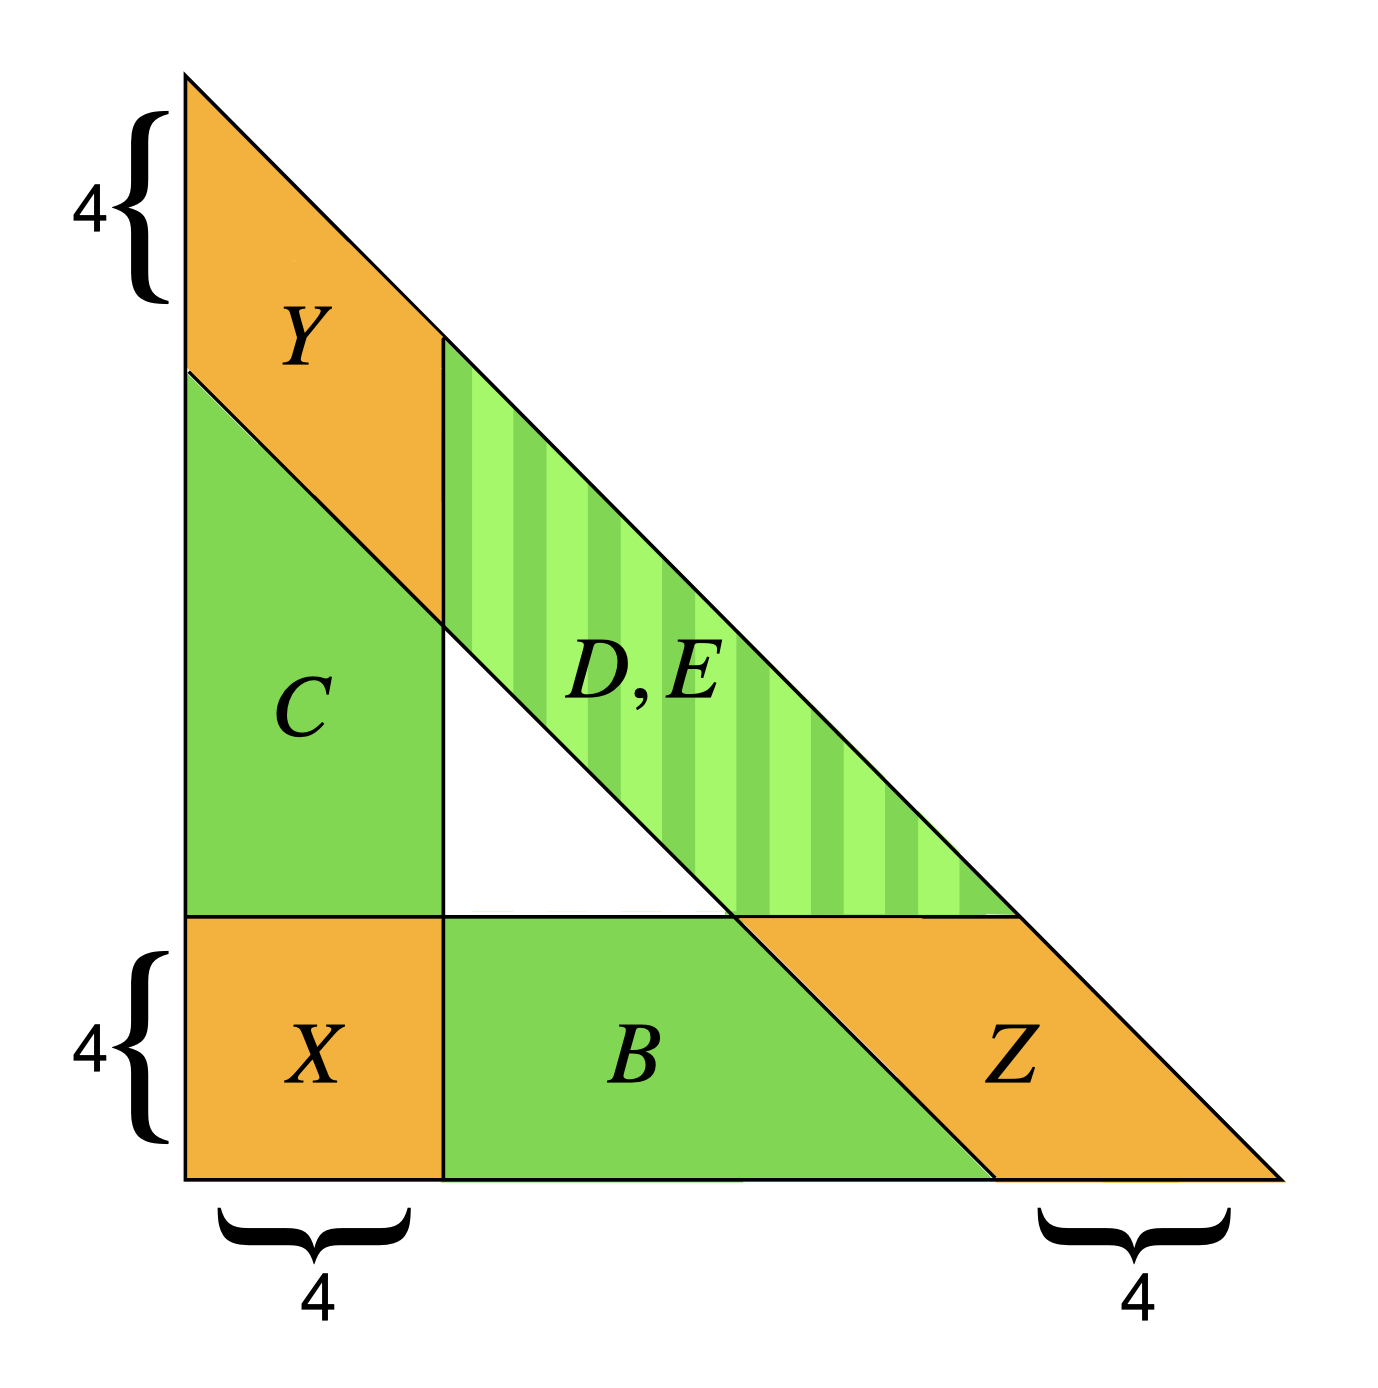
\includegraphics[width=0.75\textwidth]{assets/contactions-4.png}
    \caption{This figure illustrates the contraction variables and is taken from \cite{bik2022classifying}. The yellow areas \( X, Y, Z \) represent formal variables \( x_{i,j} \) that are unaffected by the contraction. The mint areas \( B, C, D \) represent rows and columns of vertices that are merged into a single vertex. The area \( D \) is further divided into areas \( D_1, D_2 \) by alternating columns.}
\end{figure}

\begin{definition}\label{def:contraction-variables}
Let \( x_{i,j} \) be formal variables indexed by \( V_d \). We merge a subset of rows and columns of formal variables \( x_{i,j} \) in \( V_d \) into a single vertex by defining the following \emph{contraction variables}:
\begin{align*}
    y_{i,j} &\coloneqq x_{i, d-3-i+j} \quad \text{ for } i,j = 0, \dots, 3, \\
    z_{i,j} &\coloneqq x_{d-3-j+i,j} \quad \text{ for } i,j = 0, \dots, 3, \\
    b_j &\coloneqq x_{4,j} + \dots + x_{d-4-j,j} \quad \text{ for } j = 0, \dots, 3, \\
    c_i &\coloneqq x_{i,4} + \dots + x_{i,d-4-i} \quad \text{ for } i = 0, \dots, 3, \\
    d_k &\coloneqq \begin{cases}
        x_{4,d-4-k} + x_{6,d-6-k} + \dots + x_{d-4-k,4} & \text{ if \( d + k \) is even} \\
        x_{4,d-4-k} + x_{6,d-6-k} + \dots + x_{d-5-k,5} & \text{ if \( d + k \) is odd}
    \end{cases} \quad \text{ for } k = 0, \dots, 3, \\
    e_k &\coloneqq \begin{cases}
        x_{5,d-5-k} + x_{7,d-7-k} + \dots + x_{d-5-k,5} & \text{ if \( d + k \) is even} \\
        x_{5,d-5-k} + x_{7,d-7-k} + \dots + x_{d-4-k,4} & \text{ if \( d + k \) is odd}
    \end{cases} \quad \text{ for } k = 0, \dots, 3.
\end{align*}
\end{definition}

Let us visualize the contraction variables for \( d = 16 \) in the following figure.

\begin{figure}[H]
    \begin{align*}
        \begin{array}{cccccccccccccccccccc}
            y_{0,3} & & & & & & & & & & & & \\
            y_{0,2} & y_{1,3} & & & & & & & & & & & \\
            y_{0,1} & y_{1,2} & y_{2,3} & & & & & & & & & & \\
            y_{0,0} & y_{1,1} & y_{2,2} & y_{3,3} & & & & & & & & & \\
            c_0 & y_{1,0} & y_{2,1} & y_{3,2} & d_0 & & & & & & & & \\
            c_0 & c_1 & y_{2,0} & y_{3,1} & d_1 & e_0 & & & & & & & \\
            c_0 & c_1 & c_2 & y_{3,0} & d_2 & e_1 & d_0 & & & & & & \\
            c_0 & c_1 & c_2 & c_3 & d_3 & e_2 & d_1 & e_0 & & & & & \\
            c_0 & c_1 & c_2 & c_3 &  *  & e_3 & d_2 & e_1 & d_0 & & & & \\
            c_0 & c_1 & c_2 & c_3 &  *  & * & d_3 & e_2 & d_1 & e_0 & & & \\
            c_0 & c_1 & c_2 & c_3 &  *  & * & * & e_3 & d_2 & e_1 & d_0 & & \\
            c_0 & c_1 & c_2 & c_3 &  *  & * & * & * & d_3 & e_2 & d_1 & e_0 & \\
            c_0 & c_1 & c_2 & c_3 &  *  & * & * & * & * & e_3 & d_2 & e_1 & d_0 \\
            x_{0,3} & x_{1,3} & x_{2,3} & x_{3,3} & b_3 & b_3 & b_3 & b_3 & b_3 & b_3 & z_{0,3} & z_{1,3} & z_{2,3} & z_{3,3} \\
            x_{0,2} & x_{1,2} & x_{2,2} & x_{3,2} & b_2 & b_2 & b_2 & b_2 & b_2 & b_2 & b_2 & z_{0,2} & z_{1,2} & z_{2,2} & z_{3,2} \\
            x_{0,1} & x_{1,1} & x_{2,1} & x_{3,1} & b_1 & b_1 & b_1 & b_1 & b_1 & b_1 & b_1 & b_1 & z_{0,1} & z_{1,1} & z_{2,1} & z_{3,1} \\
            x_{0,0} & x_{1,0} & x_{2,0} & x_{3,0} & b_0 & b_0 & b_0 & b_0 & b_0 & b_0 & b_0 & b_0 & b_0 & z_{0,0} & z_{1,0} & z_{2,0} & z_{3,0}
        \end{array}
    \end{align*}  
    \caption{Contraction variables for \( d = 16 \) are depicted.}
\end{figure}

As we can see, the vertices \( x_{0,4}, \dots, x_{0, d-4} \) are merged into the contraction variable \( c_0 \) by summing them up. Similarly, the formal variables \( x_{i,4}, \dots, x_{i,d-4-i} \) are merged into \( c_i \) for \( i = 1,2,3 \).

We remind that hyperfield Pascal forms are expressed as sums \( \sum_{(i,j) \in V_d} \lambda_{i,j} x_{i,j} \) with \( \lambda_{i,j} \in H \). The key insight is that there are some Pascal forms that can be expressed in terms of the contraction variables \( c_0 , c_1, c_2\) and \( c_3 \) instead of the original variables \( x_{i,j} \) for all vertices \( (i,j) \) in the \( C \)-area of Figure \ref{fig:contractions-42342432}.

\begin{example}
    Consider the Pascal form \( \mathrm{diag}(1) \) in \( \mathbb{Z}^{V_{16}} \). Its support is depicted in the following figure:
    \begin{verbatim}
        .
        +  +
        +  +  . 
        +  +  .  .  
        +  +  .  .  .  
        +  +  .  .  .  .  
        +  +  .  .  .  .  .  
        +  +  .  .  .  .  .  .  
        +  +  .  .  .  .  .  .  .
        +  +  .  .  .  .  .  .  .  .  
        +  +  .  .  .  .  .  .  .  .  .
        +  +  .  .  .  .  .  .  .  .  .  .
        +  +  .  .  .  .  .  .  .  .  .  .  .
        +  +  .  .  .  .  .  .  .  .  .  .  .  .
        +  +  .  .  .  .  .  .  .  .  .  .  .  .  .
        +  +  .  .  .  .  .  .  .  .  .  .  .  .  .  .
        +  +  .  .  .  .  .  .  .  .  .  .  .  .  .  .  .
    \end{verbatim}
    We see that \( \mathrm{diag}(1) = x_{0,0} + x_{0,1} + x_{0,2} + x_{0,3} + x_{1,0} + x_{1,1} + x_{1,2} + x_{1,3} + y_{0,0} + y_{0,1} + y_{0,2} + y_{1,0} + y_{1,1} + y_{1,2} + y_{1,3} + c_0 + c_1\).
\end{example}

The previous example also demonstrates that the expression \( \mathrm{diag}(1) = x_{0,0} + x_{0,1} + x_{0,2} + x_{0,3} + x_{1,0} + x_{1,1} + x_{1,2} + x_{1,3} + y_{0,0} + y_{0,1} + y_{0,2} + y_{1,0} + y_{1,1} + y_{1,2} + y_{1,3} + c_0 + c_1 \) is \emph{independent} of the degree \( d \), i.e. if we were to consider the Pascal form \( \mathrm{diag}(1) \) in \( \mathbb{Z}^{V_{d}} \) for some arbitrary \( d \), the expression would still hold. This is great news since it allows us to express Pascal forms in terms of contraction variables for all degrees \( d \) at once.

So far, we have only considered the contraction variables \( c_0, c_1, c_2 \), and \( c_3 \). As we might expect, we can also express some Pascal forms in terms of the contraction variables \( b_0, b_1, b_2, b_3 \), \( d_0, d_1, d_2, d_3 \), \( e_0, e_1, e_2, e_3 \), \( y_{i,j} \), and \( z_{i,j} \). We will now find these kinds of Pascal forms that can be represented in terms of the contraction variables independent of the degree \( d \). A good set of Pascal forms to consider are the Pascal forms \( \mathrm{diag}(k),  \mathrm{col}(k) \) and \( \mathrm{row}(k) \) for \( k = 0,1,2,3,d-3,d-2,d-1,d \).

\begin{proposition}\label{prop:contracted-part-1}
    Let \( d \geq 11 \). Let \( p \) be a hyperfield form induced by one of the following Pascal forms on \( \mathbb{Z}^{V_d} \):
    \begin{enumerate}
        \item \( \mathrm{col}(1), \mathrm{col}(2), \mathrm{col}(3) \), or
        \item \( \mathrm{row}(1), \mathrm{row}(2), \mathrm{row}(3)\), or
        \item \( \mathrm{diag}(1), \mathrm{diag}(2), \mathrm{diag}(3) \), or
        \item \( \mathrm{diag}(d-1), \mathrm{diag}(d-2), \mathrm{diag}(d-3) \).
    \end{enumerate}
    Then, we have 
    \begin{align*}
        p = \sum_{i,j = 0}^3 \lambda_{i,j}^{(x)} x_{i,j} + \sum_{i,j = 0}^3 \lambda_{i,j}^{(y)} y_{i,j} + \sum_{i,j = 0}^3 \lambda_{i,j}^{(z)} z_{i,j} + \sum_{j=0}^3 \lambda_{j}^{(b)} b_j + \sum_{i=0}^3 \lambda_{i}^{(c)} c_i + \sum_{k=0}^3 \lambda_{k}^{(d)} d_k + \sum_{k=0}^3 \lambda_{k}^{(e)} e_k
    \end{align*}
    with coefficients \( \lambda_{i,j}^{(x)}, \lambda_{i,j}^{(y)}, \lambda_{i,j}^{(z)}, \lambda_{j}^{(b)}, \lambda_{i}^{(c)}, \lambda_{k}^{(d)}, \lambda_{k}^{(e)} \in H \).
    
    Define \( \lambda(p,d) \coloneqq \left(\lambda_{i,j}^{(x)}, \lambda_{i,j}^{(y)}, \lambda_{i,j}^{(z)}, \lambda_{j}^{(b)}, \lambda_{i}^{(c)}, \lambda_{k}^{(d)}, \lambda_{k}^{(e)} \right) \) for the coefficients of \( p \) on \( H^{V_d} \). Then, we have
    \begin{align*}
        \lambda(p,d) &= \lambda(p,d+1) = \lambda(p,d+2) = \lambda(p,d+3) = \dots
    \end{align*}
    In other words, all the coefficients  \( \lambda_{i,j}^{(x)}, \lambda_{i,j}^{(y)}, \lambda_{i,j}^{(z)}, \lambda_{j}^{(b)}, \lambda_{i}^{(c)}, \lambda_{k}^{(d)}, \lambda_{k}^{(e)} \) are independent of the degree \( d \).
\end{proposition}

\begin{proof}
    For case two and three we observe that the hyperfield form \( p \) has support contained in the areas \( X, C \), and \( Y \) from Figure \ref{fig:contractions-42342432}. This follows directly from Proposition \ref{skdmldskfmksdej}. We also see that \( p \) depends only on the column sums on \( C \).

    For case one and four we see that \( p \) has support contained in the areas \( X, B \), and \( Z \) from Figure \ref{fig:contractions-42342432} by Proposition \ref{skdmldskfmksdej}. We conclude that \( p \) depends only on the row sums on \( B \).
\end{proof}

Here is another example.

\begin{example}
    Consider \( \mathrm{diag}(3) \) and \( d = 11 \).
    \begin{verbatim}
        · 
        · · 
        · · · 
        + + + + 
        + + + + · 
        + + + + · · 
        + + + + · · · 
        + + + + · · · · 
        + + + + · · · · · 
        + + + + · · · · · · 
        + + + + · · · · · · · 
        + + + + · · · · · · · ·
    \end{verbatim}
    Write 
    \begin{align*}
        \mathrm{sign}(\mathrm{diag}(3)) = \sum_{i,j=0}^3 x_{i,j} + \sum_{i=0}^3 c_i + \sum_{i=0}^3 \sum^{i}_{j=0} y_{i,j}.
    \end{align*}
    This linear form is independent of the degree \( d \).
\end{example}


\begin{proposition}\label{prop:contracted-part-2}
    Let \( d \geq 12 \). Let \( p \) be a hyperfield form induced by one of the following Pascal forms on \( \mathbb{Z}^{V_d} \):
    \begin{enumerate}
        \item \( \mathrm{col}(d), \mathrm{col}(d-1), \mathrm{col}(d-2), \mathrm{col}(d-3) \), or
        \item \( \mathrm{row}(d), \mathrm{row}(d-1), \mathrm{row}(d-2), \mathrm{row}(d-3)\).
    \end{enumerate}
    Then, we have 
    \begin{align*}
        p = \sum_{i,j = 0}^3 \lambda_{i,j}^{(x)} x_{i,j} + \sum_{i,j = 0}^3 \lambda_{i,j}^{(y)} y_{i,j} + \sum_{i,j = 0}^3 \lambda_{i,j}^{(z)} z_{i,j} + \sum_{j=0}^3 \lambda_{j}^{(b)} b_j + \sum_{i=0}^3 \lambda_{i}^{(c)} c_i + \sum_{k=0}^3 \lambda_{k}^{(d)} d_k + \sum_{k=0}^3 \lambda_{k}^{(e)} e_k
    \end{align*}
    with coefficients \( \lambda_{i,j}^{(x)}, \lambda_{i,j}^{(y)}, \lambda_{i,j}^{(z)}, \lambda_{j}^{(b)}, \lambda_{i}^{(c)}, \lambda_{k}^{(d)}, \lambda_{k}^{(e)} \in H \).
    
    Define \( \lambda(p,d) \coloneqq \left(\lambda_{i,j}^{(x)}, \lambda_{i,j}^{(y)}, \lambda_{i,j}^{(z)}, \lambda_{j}^{(b)}, \lambda_{i}^{(c)}, \lambda_{k}^{(d)}, \lambda_{k}^{(e)} \right) \) for the coefficients of \( p \) on \( H^{V_d} \). Then, we have
    \begin{align*}
        \lambda(p,d) &= \lambda(p,d+2) = \lambda(p,d+4) = \lambda(p,d+6) = \dots \\
        \lambda(p,d+1) &= \lambda(p,d+3) = \lambda(p,d+5) = \lambda(p,d+7) = \dots 
    \end{align*}
    In other words, all the coefficients of forms on even degrees are independent, and all the coefficients of forms on odd degrees are independent of the degree \( d \).
\end{proposition}

\begin{proof}
    All the hyperfield forms \( p \) depend on entries in the area \( Y, D \), and \( Z \) from Figure \ref{fig:contractions-42342432} by Proposition \ref{skdmldskfmksdej}. We see that \( p \) depends only on the alternating diagonal sums on \( D \) for \( x_{i,j} \) in the area \( D \). This shows that \( p \) is a sum of the contraction variables \( y_{i,j} \), \( z_{i,j} \), and \( d_k - e_k \).
\end{proof}

\begin{example}
    Consider \( \mathrm{col}(d-3) \). Let \( d = 12 \). The support of \( \mathrm{sign}(\mathrm{col}(d-3)) \) is depicted in the following figure:
    \begin{verbatim}
        · 
        · · 
        · · · 
        + + + + 
        · - - - - 
        · · + + + + 
        · · · - - - - 
        · · · · + + + + 
        · · · · · - - - - 
        · · · · · · + + + + 
        · · · · · · · - - - - 
        · · · · · · · · + + + + 
        · · · · · · · · · - - - -
    \end{verbatim}
    We write 
    \begin{align*}
        \mathrm{sign}(\mathrm{col}(d-3)) = \sum^3_{i=0}\sum^i_{j=0} (-1)^{i+j}y_{i,j} - \sum^3_{k=0}(-1)^{k}d_k  + \sum^3_{k=0}(-1)^{k}e_k - \sum^3_{i,j=0}(-1)^{j}z_{i,j}.
    \end{align*}
    For \( d = 13 \), the support of \( \mathrm{sign}(\mathrm{col}(d-3)) \) is depicted in the following figure:
    \begin{verbatim}
        · 
        · · 
        · · · 
        + + + + 
        · - - - - 
        · · + + + + 
        · · · - - - - 
        · · · · + + + + 
        · · · · · - - - - 
        · · · · · · + + + + 
        · · · · · · · - - - - 
        · · · · · · · · + + + + 
        · · · · · · · · · - - - -
        · · · · · · · · · · + + + +
    \end{verbatim}
    We write 
    \begin{align*}
        \mathrm{sign}(\mathrm{col}(d-3)) = \sum^3_{i=0}\sum^i_{j=0} (-1)^{i+j}y_{i,j} - \sum^3_{k=0}(-1)^{k}d_k  + \sum^3_{k=0}(-1)^{k}e_k + \sum^3_{i,j=0}(-1)^{j}z_{i,j}.
    \end{align*}
\end{example}

We have merged formal variables \( x_{i,j} \) indexed by vertices \( (i,j) \) in the areas \( B, C, D \) into contraction variables. Now, we apply these contractions to concrete elements \( \mathbf{s} \in H^{V_d} \).

\begin{definition}
    Define the index set
    \begin{align*}
        \Xi \coloneqq \left\{ 0,1,2,3 \right\}^2 \sqcup \left\{ 0,1,2,3 \right\}^2 \sqcup \left\{ 0,1,2,3 \right\}^2 \sqcup \left\{ 0,1,2,3 \right\} \sqcup \left\{ 0,1,2,3 \right\} \sqcup \left\{ 0,1,2,3 \right\} \sqcup \left\{ 0,1,2,3 \right\}.
    \end{align*}
    Let \( \mathbf{s} \in H^{\Xi} \). We call \( \mathbf{s} \) a \emph{contracted hyperfield configuration}, and write \( \mathbf{s} \) as
    \begin{align*}
        \mathbf{s} = (\mathbf{x}, \mathbf{y}, \mathbf{z}, \mathbf{b}, \mathbf{c}, \mathbf{d}, \mathbf{e}) = (x_{i,j}, y_{i,j}, z_{i,j}, b_j, c_i, d_k, e_k).
    \end{align*}
\end{definition}

\begin{definition}
    Let \( \mathbf{s} \in H^{\Xi}\) be a {contracted hyperfield configuration}.
    We say \( \mathbf{s} \) is \emph{valid} if one of the following holds:
    \begin{enumerate}
        \item \( \mathbf{s} = \mathbf{0} \) or
        \item \( s_{0,0} = -1 \), \( x_{i,j} \geq 0 \) for all \( i+j > 0 \), and \(  y_{i,j}, z_{i,j}, b_j, c_i, d_k, e_k \geq 0 \) for all \( i,j,k = 0,1,2,3 \).
    \end{enumerate}
\end{definition}

Going from the world of hyperfield configurations to the world of \emph{contracted} hyperfield configurations is done via the following map.

\begin{definition}
    Let \( d \geq 11 \). Let \( \mathbf{s} \in H^{V_d} \) be a hyperfield configuration. We define 
    \begin{align*}
        \mathrm{contr}_d(\mathbf{s}): \mathbf{s} \mapsto (\mathbf{x}, \mathbf{y}, \mathbf{z}, \mathbf{b}, \mathbf{c}, \mathbf{d}, \mathbf{e}) = (x_{i,j}, y_{i,j}, z_{i,j}, b_j, c_i, d_k, e_k)
    \end{align*}
    where we set
    \begin{align*}
        x_{i,j} &\coloneqq s_{i,j} \quad \text{ for } i,j = 0, \dots, 3, \\
        y_{i,j} &\coloneqq s_{i, d-3-i+j} \quad \text{ for } i,j = 0, \dots, 3, \\
        z_{i,j} &\coloneqq s_{d-3-j+i,j} \quad \text{ for } i,j = 0, \dots, 3, \\
        b_j &\coloneqq s_{4,j} + \dots + s_{d-4-j,j} \quad \text{ for } j = 0, \dots, 3, \\
        c_i &\coloneqq s_{i,4} + \dots + s_{i,d-4-i} \quad \text{ for } i = 0, \dots, 3, \\
        d_k &\coloneqq \begin{cases}
            s_{4,d-4-k} + s_{6,d-6-k} + \dots + s_{d-4-k,4} & \text{ if \( d + k \) is even} \\
            s_{4,d-4-k} + s_{6,d-6-k} + \dots + s_{d-5-k,5} & \text{ if \( d + k \) is odd}
        \end{cases} \quad \text{ for } k = 0, \dots, 3, \\
        e_k &\coloneqq \begin{cases}
            s_{5,d-5-k} + s_{7,d-7-k} + \dots + s_{d-5-k,5} & \text{ if \( d + k \) is even} \\
            s_{5,d-5-k} + s_{7,d-7-k} + \dots + s_{d-4-k,4} & \text{ if \( d + k \) is odd}
        \end{cases} \quad \text{ for } k = 0, \dots, 3.
    \end{align*}
    exactly as in Definition \ref{def:contraction-variables}.
\end{definition}

The contraction map \( \mathrm{contr}_d \) maps hyperfield configurations \( \mathbf{s} = (\mathbf{x}, \mathbf{y}, \mathbf{z}, \mathbf{b}, \mathbf{c}, \mathbf{d}, \mathbf{e}) \in H^{{V_d}} \) to elements in \( H^{\Xi} \) if \( \mathbf{b}, \mathbf{c}, \mathbf{d}, \mathbf{e}  \geq 0\). If one of the entries is negative, the map may output to some element \( (2^H)^{\Xi} \). To make life easier, we introduce the following definition.

\begin{definition}
    Let \( \mathbf{s} \in H^{V_d} \) be a hyperfield configuration. We say \( \mathbf{s} \) is \emph{weakly valid} if for all \( (i,j) \in \mathrm{supp}^-(\mathbf{s}) \) one of the following holds:
    \begin{enumerate}
        \item \( i,j = 0, \dots, 3 \), or
        \item \( i = 0, \dots, 3 \) and \( i+j \geq d-3 \), or
        \item \( j = 0, \dots, 3 \) and \( i + j \geq d-3 \).
    \end{enumerate}
\end{definition}

\begin{figure}[H]
    \centering
    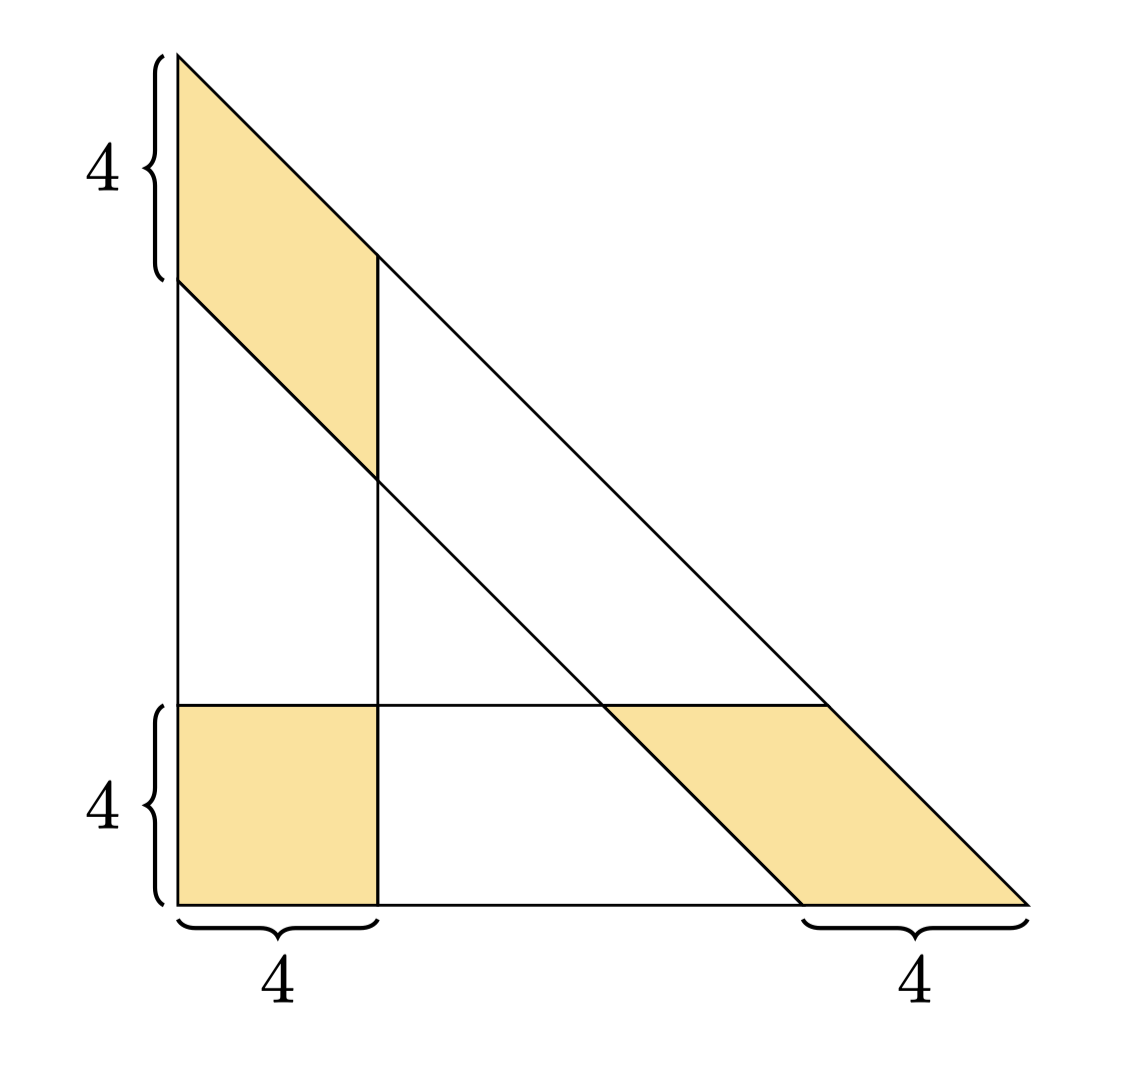
\includegraphics[width=0.75\textwidth]{assets/weakly-valid.png}
    \caption{A hyperfield configuration is weakly valid if its negative support is contained in the yellow area. The figure is taken from \cite{bik2022classifying}.}
\end{figure}

From now on, we only consider \emph{weakly valid} hyperfield configurations because in this case the contraction map \( \mathrm{contr}_d \) always outputs elements in \( H^{\Xi} \).

\begin{definition}
    Let \( \mathbf{s} \in H^{\Xi} \) be a contracted hyperfield configuration. The \emph{positive support} of \( \mathbf{s} = (\mathbf{x}, \mathbf{y}, \mathbf{z}, \mathbf{b}, \mathbf{c}, \mathbf{d}, \mathbf{e}) \) is defined as the set of all symbols \( x_{i,j}, y_{i,j}, z_{i,j}, b_j, c_i, d_k, e_k \) such that the corresponding coefficients of \( \mathbf{s} \) equal to one.
\end{definition}

\begin{example}
    Let \( \mathbf{s} = (\mathbf{x}, \mathbf{y}, \mathbf{z}, \mathbf{b}, \mathbf{c}, \mathbf{d}, \mathbf{e}) \in H^{\Xi}\) be a contracted hyperfield configuration defined by 
    \begin{align*}
        x_{0,0} = -1, \quad x_{0,3} = 1, \quad x_{1,1} = 1, \quad, x_{3,0} = 1, \quad d_0 = 1, \quad e_0 = 1
    \end{align*}
    where all other entries are zero. Then, the positive support of \( \mathbf{s} \) is given by
    \begin{align*}
        \mathrm{supp}^+(\mathbf{s}) = \left\{ x_{0,3}, x_{1,1}, x_{3,0}, d_0, e_0 \right\}.
    \end{align*}
\end{example}
